\section{Unresolved discrimination and limitations of observational criteria}
\label{sec:limitations}

\begin{wrapfigure}{r}{0.31\textwidth}
  \begin{center}
  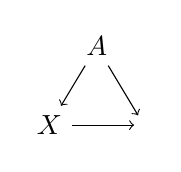
\begin{tikzpicture}
    \pgfmathsetmacro{\d}{1}
    \node (A) at (0,0) {$A$};
    \node (X) at (-0.6,-1) {$X$};
    \node (R) at (0.6,-1) {$\hR$};
    \draw[->] (A) -- (X);
    \draw[->] (A) -- (R);
    \draw[->] (X) -- (R);
  \end{tikzpicture}%
  \caption{The admission decision~$\hR$ does not only directly depend on
  gender~$A$, but also on department choice~$X$, which in turn is also
  affected by gender~$A$.}
  \label{fig:pearl}
  \end{center}
\end{wrapfigure}

To bear out the limitations of observational criteria, we turn to Pearl's
commentary on claimed gender discrimination in Berkeley college
admissions~\cite[Section 4.5.3]{Pearl2009}. Bickel~\cite{Bickel1975} had shown
earlier that a lower college-wide admission rate for women than for men was
explained by the fact that women applied in more competitive departments. When
adjusted for department choice, women experienced a slightly higher acceptance
rate compared with men. From the causal point of view, what matters is the
\emph{direct effect} of the protected attribute (here, gender~$A$) on the
decision (here, college admission~$\hR$) that cannot be ascribed to a
\emph{resolving variable} such as department choice~$X$, see \figref{fig:pearl}.
We shall use the term \emph{resolving variable} for any variable in the causal
graph that is influenced by~$A$ in a manner that we accept as
non-discriminatory. With this convention, the criterion can be stated as
follows.

\begin{definition}[Unresolved discrimination]
  A variable~$V$ in a causal graph exhibits \emph{unresolved discrimination} if
  there exists a directed path from~$A$ to~$V$ that is not blocked by a
  resolving variable and~$V$ itself is non-resolving.
\end{definition}

Pearl's commentary is consistent with what we call the \emph{skeptic viewpoint}. All paths from
the protected attribute~$A$ to $R$ are problematic, unless they are justified by
a resolving variable. The presence of unresolved discrimination in the
predictor~$R$ is worrisome and demands further scrutiny. In practice,~$R$ is not
a priori part of a given graph. Instead it is our objective to construct it as a
function of the features~$X$, some of which might be resolving. Hence we should
first look for unresolved discrimination in the features. A canonical way to
avoid unresolved discrimination in~$R$ is to only input the set of features that
do not exhibit unresolved discrimination. However, the remaining features might
be affected by non-resolving \emph{and} resolving variables. In
\secref{sec:criteria} we investigate whether one can exclusively remove
unresolved discrimination from such features. A related notion of ``explanatory
features'' in a non-causal setting was introduced in~\cite{Kamiran2013}.

\begin{wrapfigure}{r}{0.5\linewidth}
  \centering
\begin{tikzpicture}
  \pgfmathsetmacro{\d}{1}
  \node (A) at (0,0) {$A$};
  \node[thick, Green] (X1) at (\d,0) {$X_1$};
  \node (Y) at (2*\d,0) {$Y$};
  \node (X2) at (\d,-\d) {$X_2$};
  \node (R) at (\d,\d) {$\hR^*$};
  \draw[->] (A) -- (X1);
  \draw[->] (X1) -- (Y);
  \draw[->] (A) -- (X2);
  \draw[->] (X1) -- (X2);
  \draw[->] (X1) -- (R);
\end{tikzpicture}%
  \hspace{0.5cm}
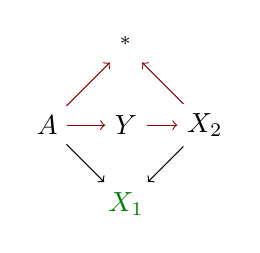
\begin{tikzpicture}
  \pgfmathsetmacro{\d}{1}
  \node (A) at (0,0) {$A$};
  \node (Y) at (\d,0) {$Y$};
  \node[thick, Green] (X1) at (\d,-\d) {$X_1$};
  \node (X2) at (2*\d,0) {$X_2$};
  \node (R) at (\d,\d) {$\hR^*$};
  \draw[->, DarkRed] (A) -- (Y);
  \draw[->, DarkRed] (Y) -- (X2);
  \draw[->, DarkRed] (X2) -- (R);
  \draw[->, DarkRed] (A) -- (R);
  \draw[->] (A) -- (X1);
  \draw[->] (X2) -- (X1);
\end{tikzpicture}%
  \caption{Two graphs that may generate the same joint distribution for the
  Bayes optimal unconstrained predictor~$\hR^*$. If~$X_1$ is a resolving
  variable,~$R^*$ exhibits unresolved discrimination in the right graph (along
  the red paths), but not in the left one.}
  \label{fig:unidentifiability}
\end{wrapfigure}

The definition of unresolved discrimination in a predictor has some interesting
special cases worth highlighting. If we take the set of resolving variables to
be empty, we intuitively get a causal analog of demographic parity. No directed paths from~$A$ to~$R$ are allowed, but~$A$ and~$R$ can
still be statistically dependent. Similarly, if we choose the set of resolving
variables to be the singleton set~$\{Y\}$ containing the true outcome, we obtain
a causal analog of equalized odds where strict independence is not necessary.
The causal intuition implied by ``the protected attribute should not affect the
prediction'', and ``the protected attribute can only affect the prediction when
the information comes through the true label'', is neglected by (conditional)
statistical independences~$A \indep R$, and~$A \indep R \given Y$, but well
captured by only considering dependences mitigated along directed causal paths.

We will next show that observational criteria are fundamentally unable to
determine whether a predictor exhibits unresolved discrimination or not. This
is true even if the predictor is \emph{Bayes optimal}. In passing, we also note that
fairness criteria such as equalized odds may or may not exhibit unresolved
discrimination, but this is again something an observational criterion cannot
determine.

\begin{theorem}\label{thm:unidentifiability}
  Given a joint distribution over the protected attribute~$A$, the true
  label~$Y$, and some features~$X_1, \dots, X_n$, in which we have already
  specified the resolving variables, no observational criterion can generally
  determine whether the Bayes optimal unconstrained predictor or the Bayes
  optimal equal odds predictor exhibit unresolved discrimination.
\end{theorem}

All proofs for the statements in this paper are in the supplementary material.

The two graphs in \figref{fig:unidentifiability} are taken
from~\cite{Hardt2016}, which we here reinterpret in the causal context to prove
Theorem~\ref{thm:unidentifiability}. We point out that there is an established
set of conditions under which unresolved discrimination can, in fact, be
determined from observational data. Note that the two graphs are not Markov
equivalent. Therefore, to obtain the same joint distribution we must violate a
condition called \emph{faithfulness}.\footnote{If we do assume the Markov
condition and faithfulness, then conditional independences determine the graph
up to its so called \emph{Markov equivalence class}.} We later argue that
violation of faithfulness is by no means pathological, but emerges naturally
when designing predictors.  In any case, interpreting conditional dependences
can be difficult in practice~\cite{Cornia2014}.
